\documentclass[a4paper,10pt,oneside,final,titlepage,onecolumn]{article}

\usepackage{ucs}
\usepackage[portuguese]{babel}
\usepackage[utf8x]{inputenc}
\usepackage[T1]{fontenc}
\usepackage{textcomp}

\usepackage{listings}
\usepackage{color}

\definecolor{dkgreen}{rgb}{0,0.6,0}
\definecolor{gray}{rgb}{0.5,0.5,0.5}
\definecolor{mauve}{rgb}{0.58,0,0.82}

\lstset{frame=tb,
  language=bash,
  aboveskip=3mm,
  belowskip=3mm,
  showstringspaces=false,
  columns=flexible,
  basicstyle={\scriptsize\ttfamily},
  numbers=none,  
  breaklines=true,
  breakatwhitespace=true
  tabsize=3
}



\title{Exercício 3 de MC833 --- Programação em Redes de Computadores}
\author{Raul Rabelo Carvalho, 105607, turma A}



\begin{document}



\maketitle



\section{htons}
\paragraph{}A função \verb|htons| faz parte de um conjunto de funções usadas para converter um inteiro, tanto de 16 bits quanto de 32 bits, entre a \emph{byte order} de rede (\emph{big endian}) e a \emph{byte order} do \emph{host} local, que pode ser \emph{big endian} ou \emph{little endian} a depender da arquitetura. É óbvio que caso a arquitetura do \emph{host} seja \emph{big endian}, nada é feito.
\paragraph{}Especificamente, a função \verb|htons| converte inteiros de 16 bits da \emph{byte order} do \emph{host} para da rede.



\section{Execução com código-fonte não-modificado}
\paragraph{}Não é possível executar o servidor sem alterações no \emph{host} do laboratório do IC (\verb|guns.ic.unicamp.br|), pois a função \verb|bind| não tem permissão para utilizar a porta 10. Esta porta é uma das \emph{well-known ports} e estão bloqueadas para usuários sem privilégios nas máquinas do IC.



\section{Resolvendo o problema do \verb|bind|}
\paragraph{}Alterando-se a porta empregada para 1234, tanto em \verb|client.c| quanto em \verb|server.c|, resolve-se o problema do servidor não conseguir reservar para si uma das \emph{well-known ports}. No entanto, o cliente não consegue se conectar a esta porta, provavelmente devido àlguma política de bloqueio de portas no roteador dos laboratórios.
\paragraph{}Fazendo uma segunda alteração para a porta 10000, o servidor consegue reservar a porta e executar normalmente, e o cliente consegue conectar-se a esta porta e cominicar-se com o servidor.
\begin{figure}[h!]
  \caption{Execução local.}
  \centering
    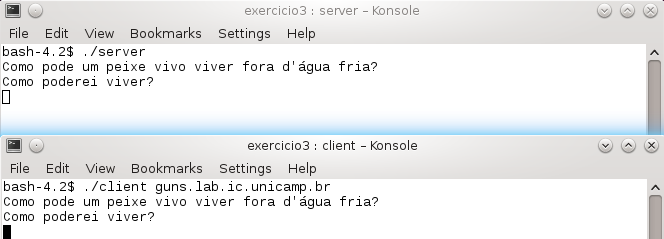
\includegraphics[width=0.5\textwidth]{exec-local.png}
\end{figure}
\paragraph{}Também foi possível executar o servidor no \emph{host} local e o cliente na máquina \verb|xaveco| via \verb|ssh|, executado com o comando \verb|./client guns.lab.ic.unicamp.br|.
\begin{figure}[h!]
  \caption{Execução remota.}
  \centering
    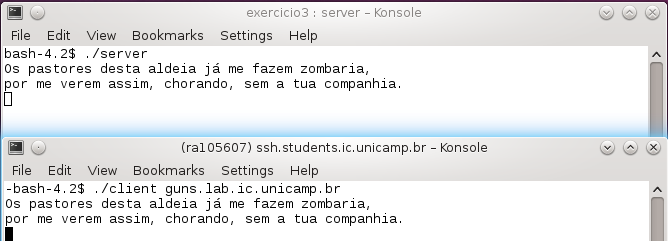
\includegraphics[width=0.5\textwidth]{exec-remota.png}
\end{figure}


\end{document}
